\documentclass[../manuscript.tex]{subfiles}
\section{Полученные результаты}
\subsection{Синтетические данные}
Обе версии алгоритма XClone хорошо показали себя на синтетических данных, полученных в соответствии с генеративными моделями. Все эксперименты воспроизводимы, т.к. при запуске обязательно нужно указать \textbf{random seed} — строку, хэш от которой инициализирует генераторы псевдослучайных чисел в коде.

Приведенные графики соответствуют валидации XClone-V1 на синтетических данных. Эксперимент был запущен с такими параметрами: 
\begin{itemize}
	\item И в ДНК-, и в РНК-модуле по 100 клеток. Это имитация протокола G\&T\cite{GTseq}: геном и транскриптом будто бы извлекается из одних и тех же клеток;
	\item Вектора $\bm{D_{j}^{G}}$ и $\bm{D_{j}^{E}}$ берутся из реальных данных;
	\item 7 клональных линий, существенно отличающихся друг от друга картиной алелльного дисбаланса — векторами $\bm{X_{k}}$;
	\item $\bm{A_{j}^{G}}$ — вектора числа прочтений материнских аллелей — результат поэлементного перемножения $ \bm{D_{j}^{G}} $ и $ \bm{X_{k}} $. Аналогично для $\bm{A_{j}^{E}}$.
	\item $10^{4}$ итераций семплирования по Гиббсу. Для стабилизации распределений на метках обычно хватало нескольких тысяч итераций, так что десяти тысяч хватало с большим запасом.
\end{itemize}
\begin{figure}[H]
	\centering
	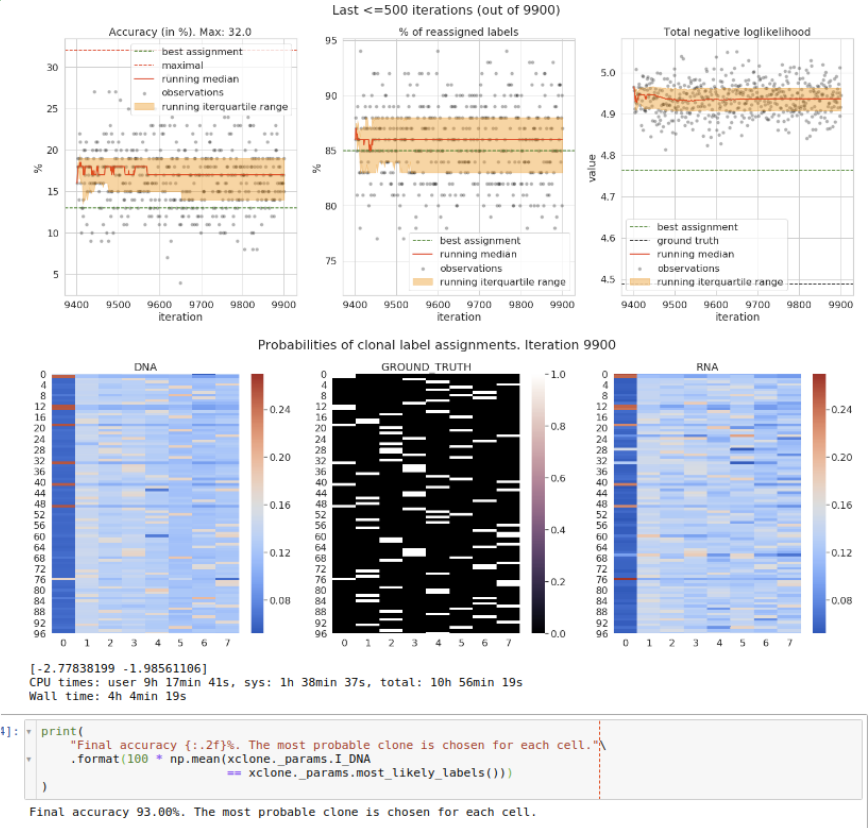
\includegraphics[keepaspectratio=true, scale=0.5]{images/xclone_v1_simulated_data_convergence_monitor.png}
	\caption{Рукописная визуализация процесса обучения XClone-V1, последние 500 итераций. Строкам тепловых карт в нижнем ряду соответствуют клетки, столбцам — клональные линии, а ячейке на позиции $(j, k)$ — вероятность того, что клетка $j$ принадлежит линии $k$. Центральная карта показывает истинные клональные линии, левая — вероятности, подсчитанные по scDNA-seq, правая — по scRNA-seq. Верхние тепловые карты позволяют, как распределения из нижних тепловых карт менялись в ходе обучения. Левая карта показывает точность предсказания, если клональная линии назначается случайно в соответствии с текущим распределением вероятностей на метках. Центральная карта показывает, какой процент меток при таком подходе отличается от расстановки, полученной 100 итераций назад. Правая карта показывает, как менялся минус логарифм функции правдподобия от итерации к итерации.}
\end{figure}

\begin{figure}[H]
	\centering
	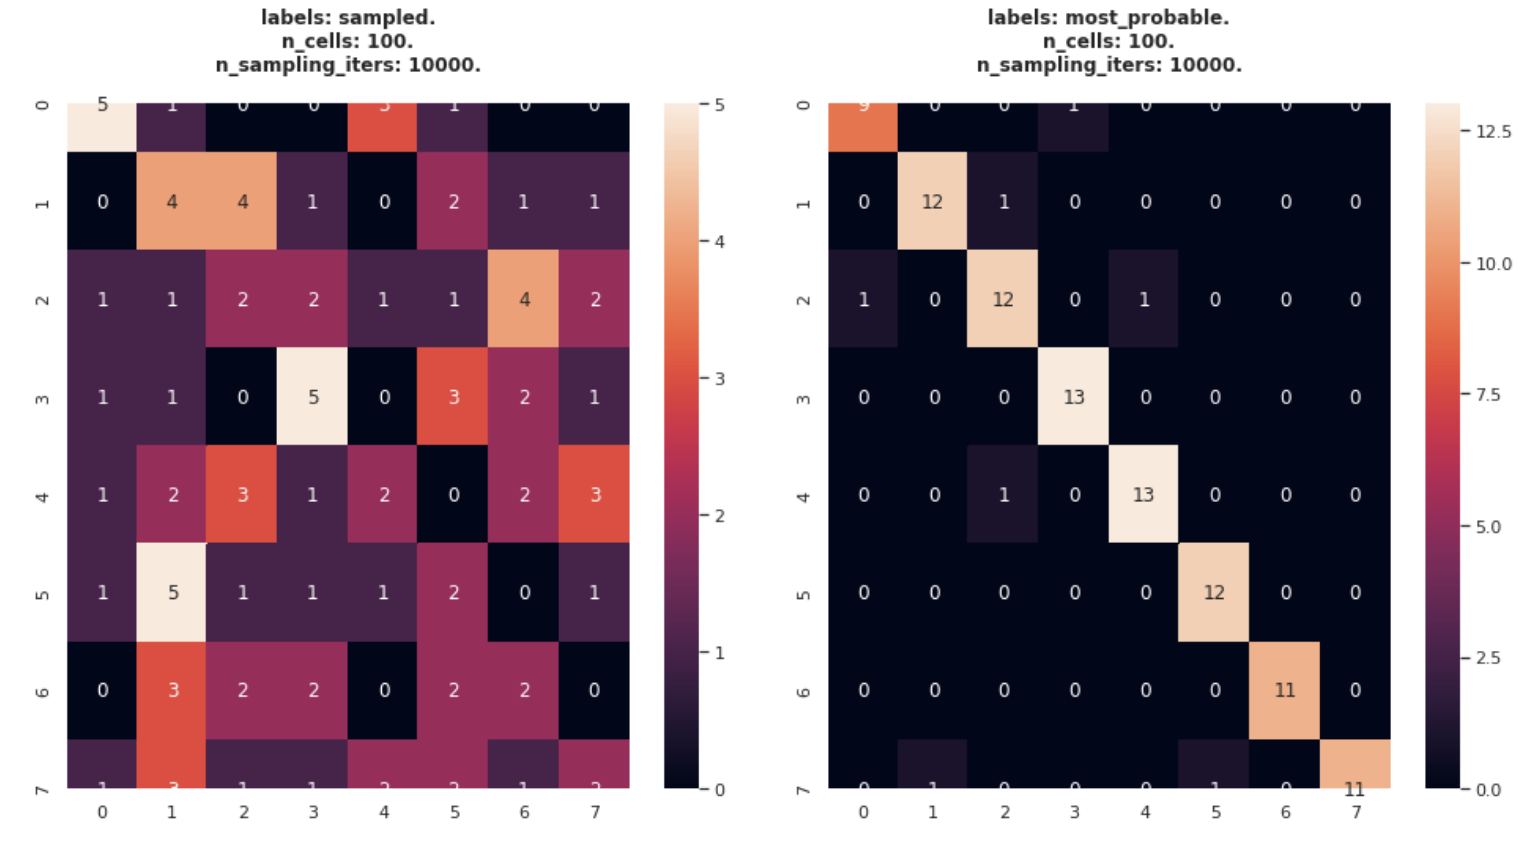
\includegraphics[keepaspectratio=true, scale=0.3]{images/xclone_v1_simulated_data_confusion_matrices.png}
	\caption{Матрицы ошибок (confusion matrix) для предсказанных клональных линий. Слева — метки, полученные семплированием, справа — моды соответствующих распределений.}
\end{figure}
По графикам видно, что алгоритм находит правильные метки, но не очень уверен в них. С ростом глубины покрытия при генерции клеток эта проблема становилась менее выраженной, но и синтетические данные при этом всё меньше напоминали реальные. Симуляция показала, что для надёжной работы алгоритма нужны были РНК-данные гораздо более высокого качества, чем в образцах от DKFZ. Кроме того, итоговая точность сильно зависела от качества BAF-сигнала, который в РНК-образцах раз за разом оказывался слишком зашумленным. Именно в связи с этим и была разработана XClone-V2, где во главе угла не BAF, а RDR.

Эксперименты для валидации XClone-V2 устроен аналогично, разве что добавляется информация о числе всех прочтений $\bm{R_{j}}$. Кроме того, теперь нужно генерировать ASCNV. Доля затронутых ими блоков сегментации в каждом из клонов задаётся пользователем, равно как и частоты отдельных аллель-специфических конфигураций $(c_{t,m}, c_{t,p})$. 
\begin{figure}[H]
	\centering
	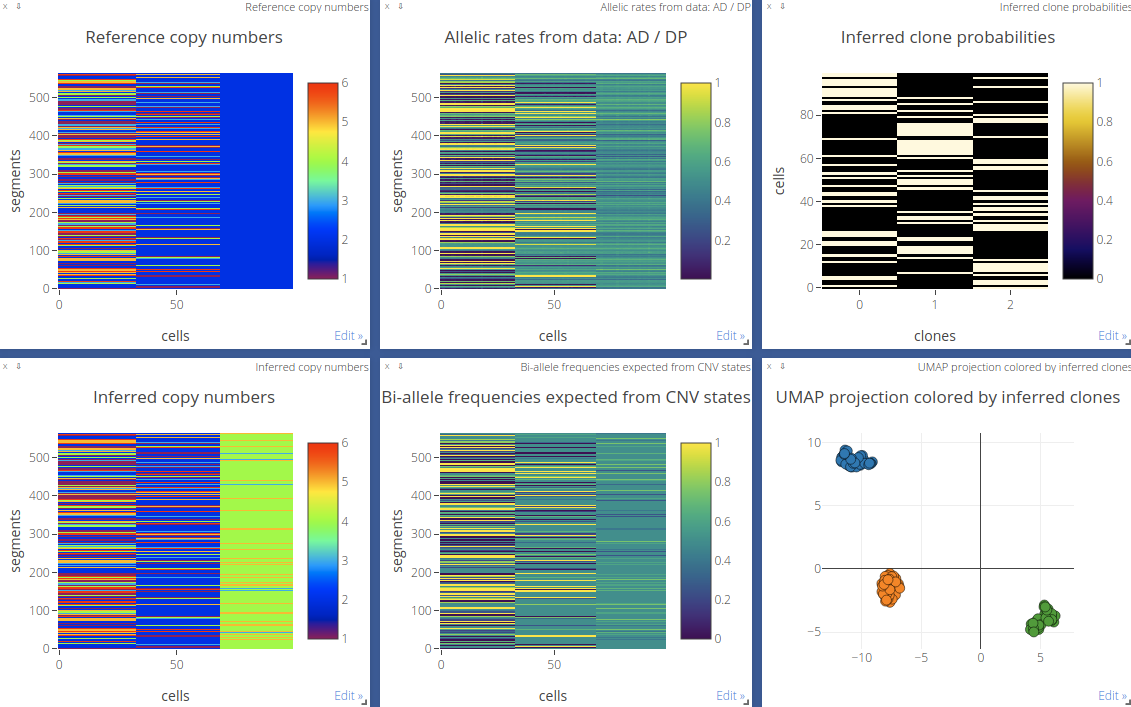
\includegraphics[keepaspectratio=true, scale=0.4]{images/xclone_v2_simulation_results.png}
	\caption{Визуализация процесса обучения XClone-V2, выполненная в Visdom от Facebook Research. Тепловые карты в верхней строке, слева направо: истинные клональные RDR- и BAF-сигналы, а также вероятности принадлежности клеток клональным линиям (все сошлись к истинным). Нижняя строка, слева направо: предсказанное число копий в каждом из клонов, предсказанный аллельный дисбаланс и проекция клеток конкатенации этих двух векторов на 2D с помощью алгоритма UMAP, где каждый цвет соответствует клональной линии.}
\end{figure}
Скачок качества очевиден: корректное распределение на метках клональных линий удаётся получить всего за пару десятков итераций VB, чего в XClone-V1 не удавалось достичь даже за 10000 итераций семплирования по Гиббсу.

При этом бросается в глаза, что модель сильно ошибается на нормальных клетках: она предсказывает WGD там, где его нет. Но ранее упоминалось, что мультиномиальная модель RDR-модуля в XClone-V2 не позволяет детектировать WGD, потому на стадии байесовского вывода такие ошибки неизбежны. Их можно попытаться скорректировать на стадии пост-обработки, об этом можно прочесть в заключительном разделе ВКР. В остальном же и BAF-, и RDR-модуль предсказывают корректные величины.

Кроме того, справедливо будет заметить, что пока что эксперименты не позволяют оценить качество модели как классификатора. В идеальных условиях незашумленных BAF- и RDR-сигналов в данных классифицировать клетки просто: видно, что клональные линии линейно разделимы при проекции на 2D. Алгоритм KMeans в таком случае тоже даёт 100\% точность. Поэтому симуляции сейчас проверяют не то, как классифицируются клетки, а как модель восстанавливает ASCNV. Сейчас это не первоочередная задача, но в последующих версиях модели будут реализованы и более продвинутые подходы к генерации данных. 

\subsection{Реальные данные: STP, scDNA-seq}
Перед тем, как перейти к рассмотрению результатов, полученных XClone-V2 на данных STP-Nuclei, стоит взглянуть на данные поближе. Дизайн XClone-V2 был вдохновлён двумя важными наблюдениями, полученными из реальных данных. 

Во первых, разработанный метод коррекции ошибок смены цепи показал, что по данным scDNA-seq можно получить надёжный BAF-сигнал. На данный момент ни один опубликованный метод, кроме CHISEL\cite{ChiselBiorxiv}, не может этим похвастать.

\begin{figure}[H]
	\centering
	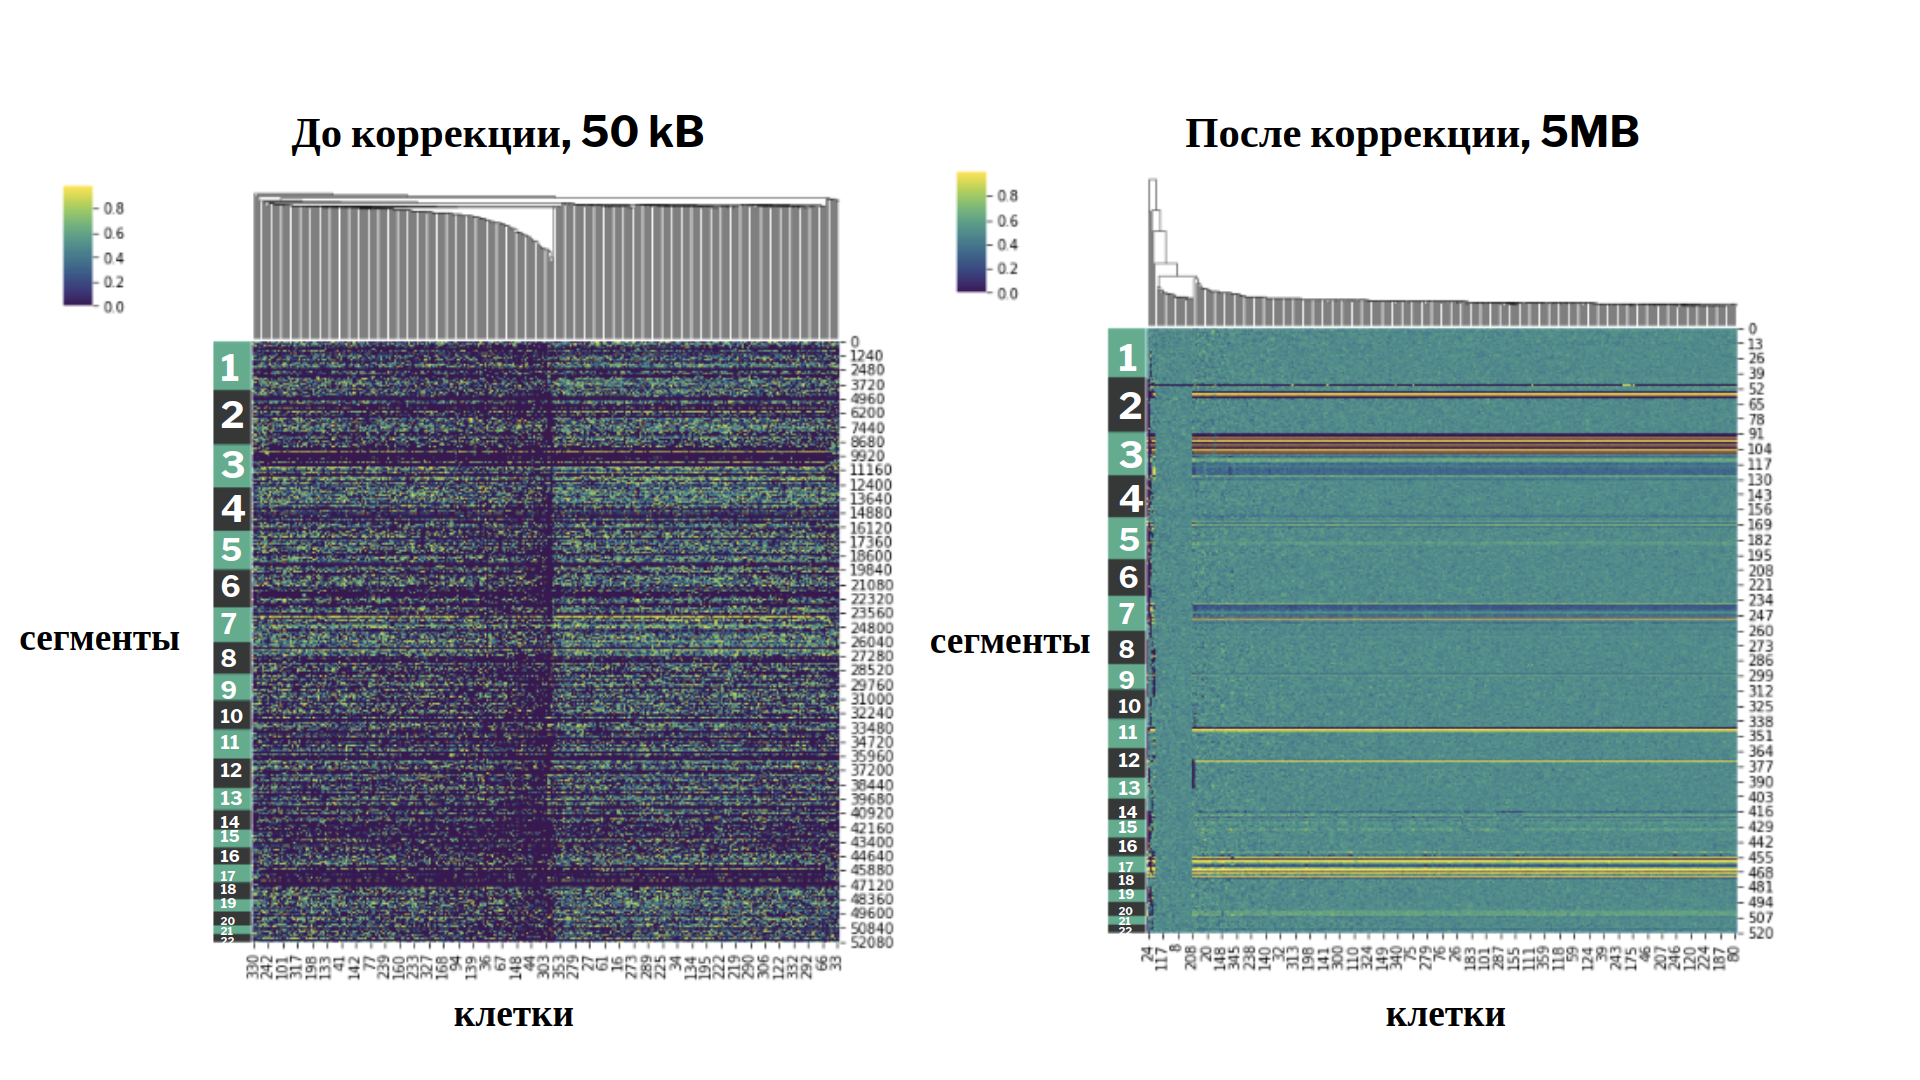
\includegraphics[keepaspectratio=true,scale=0.25]{images/bin_linkage_stp_nuclei_dna.png}
	\caption{Коррекция ошибок смены цепи на примере ДНК-образца медуллобластомы, STP-Nuclei. На рисунке изображены тепловые карты долей аллеля из <<материнского>> гаплотипа, числа слева обозначают номер хромосомы.}
\end{figure}

Картина аллельного дисбаланса до коррекции практически не прослеживается, после — становится очевидна. Видно, что при текущем подходе к сегментации теряются сложные структурные вариации в духе хромотрипсиса на хромосоме 7. Это известный недостаток, который будет устранён в следующих версиях XClone: при объединении первичных сегментов длиной 50кБ будет играть роль их взаимное подобие.

\begin{figure}[H]
	\centering
	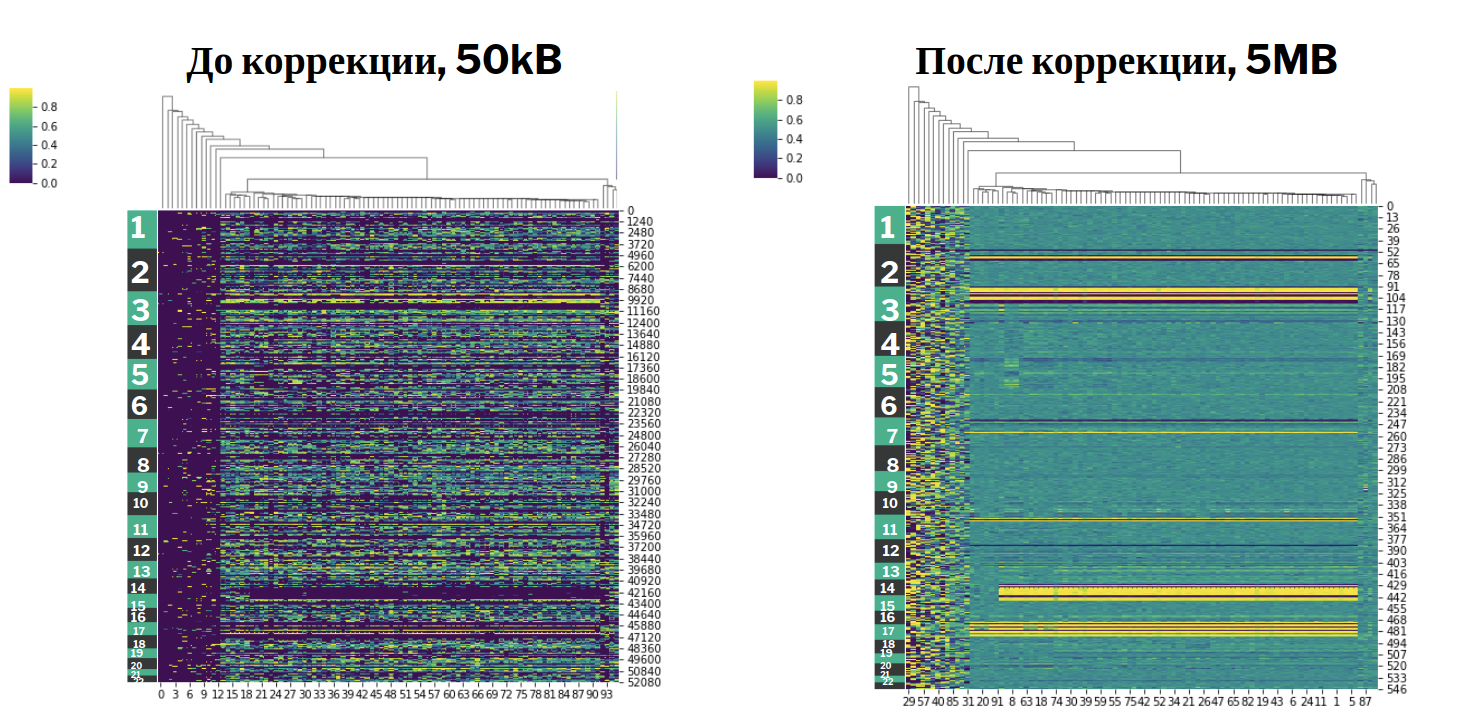
\includegraphics[keepaspectratio=true,scale=0.3]{images/bin_linkage_stp_gt_dna.png}
	\caption{Коррекция ошибок смены цепи на примере ДНК-образца медуллобластомы, STP-G\&T. Суть та же, что и на предыдущей иллюстрации, но в этом образце глубина покрытия клеток в среднем выше, а потому аллельный сигнал проступает и в масштабе 50 килобаз.}
\end{figure}

Видно, что в образце STP-G\&T гораздо отчётливее проступает большая делеция q-плеча 14-й хромосомы и p-плеча 15-й. Причём в части клеток этой делеции нет, и это может быть субклон. В STP-Nuclei весь сигнал, приходящий с 14 хромосомы, сильно размыт. Занимательно, что он прослеживается в транскриптомных данных, как это будет показано в следующем разделе. Но при этом в STP-G\&T довольно существенная доля мёртвых клеток, а сам образец в два с половиной раза меньше, потому эксперименты было решено проводит на STP-Nuclei. А два там клона или три уже было не так важно. Эта опухоль в обоих случаях слишком однородная для того, чтобы использовать её при последующей публикации статьи, а переговоры по получению более интересных образцов пока ещё не завершены.

Полученная картина аллельного дисбаланса в образце согласовывалась с априорными знаниями врачей об этой опухоли. Это позволило перейти к следующему шагу: проверке пришедшей от биологов гипотезы о том, что изменение глубины покрытия отдельных сегментов пропорционально, в первую очередь, числу копий этих участков, а остальными факторами можно пренебречь. В матрице числа прочтений обнаруживается та же структура: однородная опухоль с небольшой примесью здоровых клеток.

\begin{figure}[H]
	\centering
	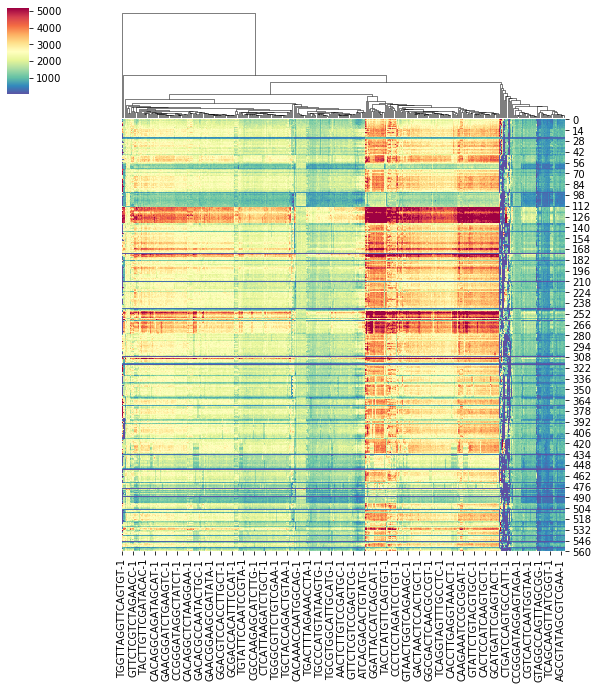
\includegraphics[keepaspectratio=true,scale=.6]{images/stp_nuclei_read_count_matrix.png}
	\caption{Матрица числа прочтений. STP-Nuclei, scDNA-seq. Cтроки — сегменты длины в 5 мегабаз, столбцы — клетки.}
\end{figure}

Видно, что среднее количество прочтений сильно меняется от клетки к клетке: есть как плохие (возможно, мёртвые) клетки (на тепловой карте справа), так и очень хорошие (оранжево-красная полоса на тепловой карте справа). Тем не менее, непохоже, что клетки с малой глубиной покрытия это отдельная клональная линия: распределение прочтений по сегментам там такое же, как и в остальных клетках. Также непохоже, что наблюдаемая субпопуляция клеток с большой глубиной покрытия это отдельная клональная линия, в которой произошло на 1 WGD больше: глубина больше, но не в степень двойки раз (50000 против 40000 это в пределах погрешности). 

\begin{figure}[H]
		\centering
	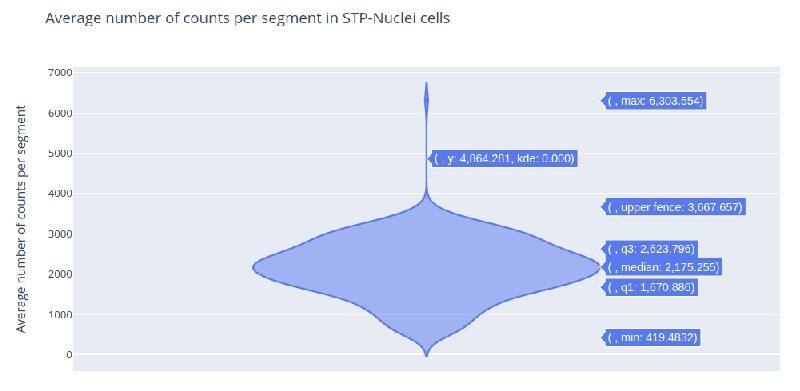
\includegraphics[keepaspectratio=true,scale=.6]{images/stp_nuclei_reads_per_segment_on_average.png}
	\caption{Распределение среднего числа прочтений в сегменте. STP-Nuclei, scDNA-seq.}
\end{figure}

Гипотеза, что по распределению прочтений по геному можно точно предсказать число копий, можно проверить, сравнив наблюдаемое в клетке $i$ распределение прочтений по сегментам с ожидаемым — 
$$
	\left\{\frac{ m_i c_{i,j} / 2 }{ \sum_{b=1}^{N} m_b c_{b,j} / 2 }\right\}_{i=1}^{N}
$$ 
где $N$ — число сегментов, $m_{i}$ — ожидаемая доля прочтений в сегменте $i$ в нормальных клетках, а $c_{i,j}$ — предсказанное число копий (нужно поделить на 2, т.к. в норме геном диплоидный).

\begin{figure}[H]
	\centering
	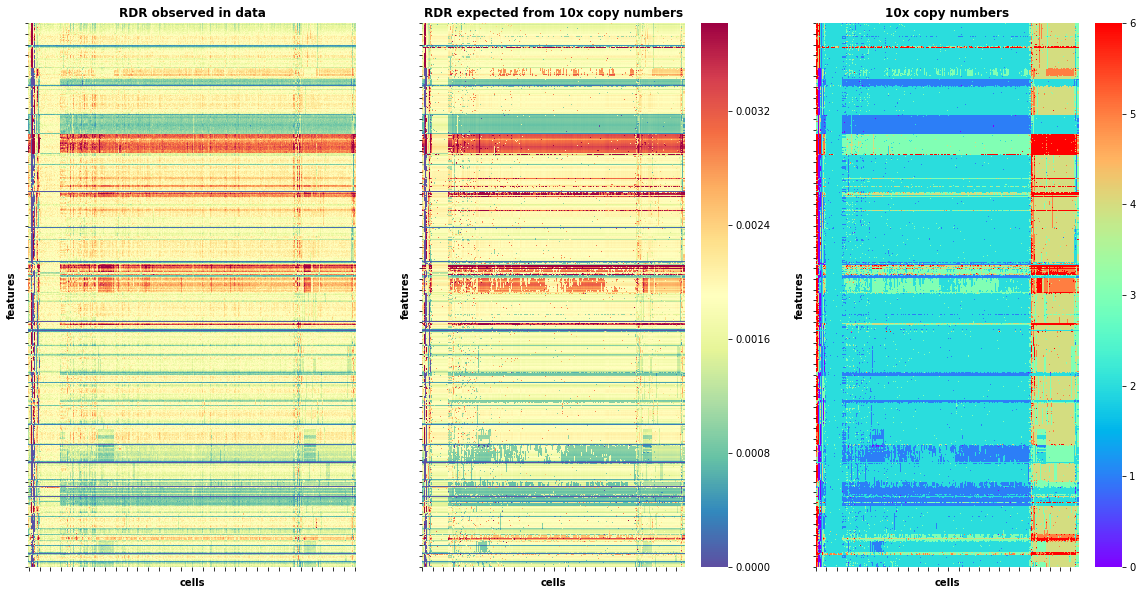
\includegraphics[keepaspectratio=true,scale=.4]{images/stp_nuclei_rdr_comparative_analysis.png}
	\caption{Распределение прочтений по геному. STP-Nuclei, scDNA-seq. Первые две тепловые карты показывают наблюдаемую долю прочтений и ожидаемую по предсказанному алгоритмом CellRanger числу копий, которое само по себе изображено на третьей тепловой карте.}
\end{figure}

Видно, что распределения, в целом, похожи. Более детальный анализ каждой из хромосом в отдельности подтверждает первое впечатление:

\begin{figure}[H]
	\centering
	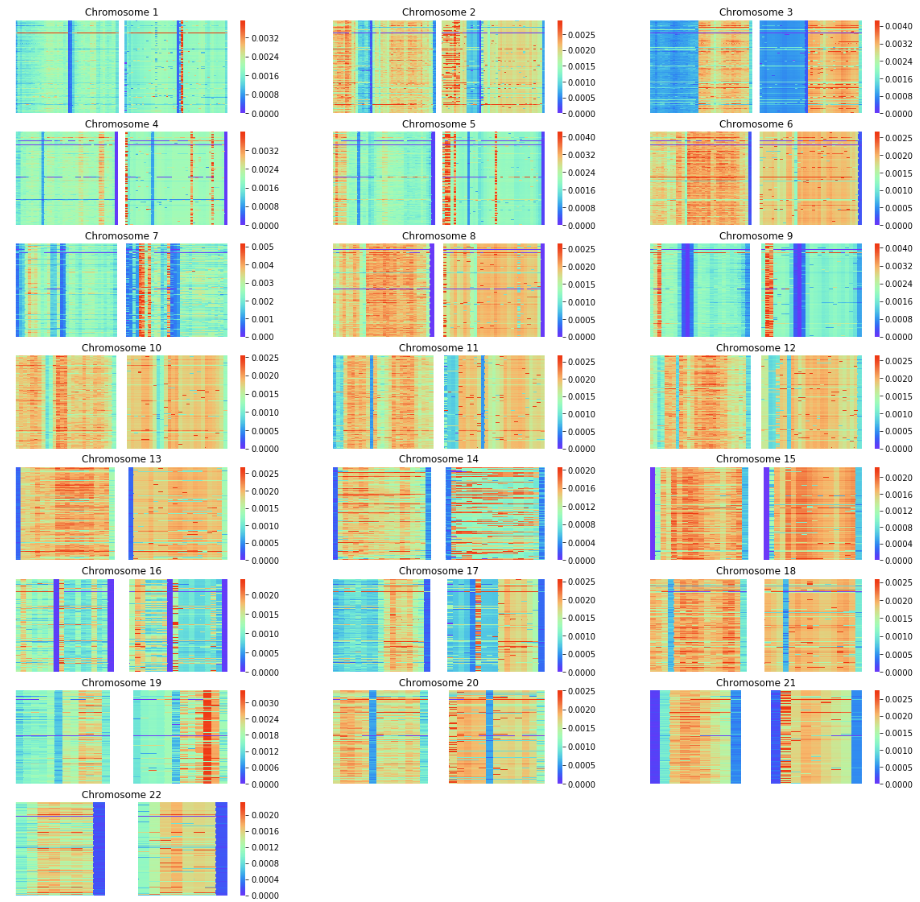
\includegraphics[keepaspectratio=true,scale=.5]{images/stp_nuclei_rdr_comparative_analysis_per_choromosome.png}
	\caption{Распределение прочтений по каждой из хросомом в отдельности. STP-Nuclei, scDNA-seq. Слева — доли прочтений, подсчитанные по реальным данным, справа — доли прочтений, ожидаемые на основе числа копий, предсказанных CellRanger.}
\end{figure}

Как уже отмечалось ранее, есть основания полагать, что диплоидные с точки зрения CellRanger клетки опухоли всё-таки тетраплоидные: глубина покрытия в этой группе клеток меньше нестатзначимо.

\begin{figure}[H]
	\centering
	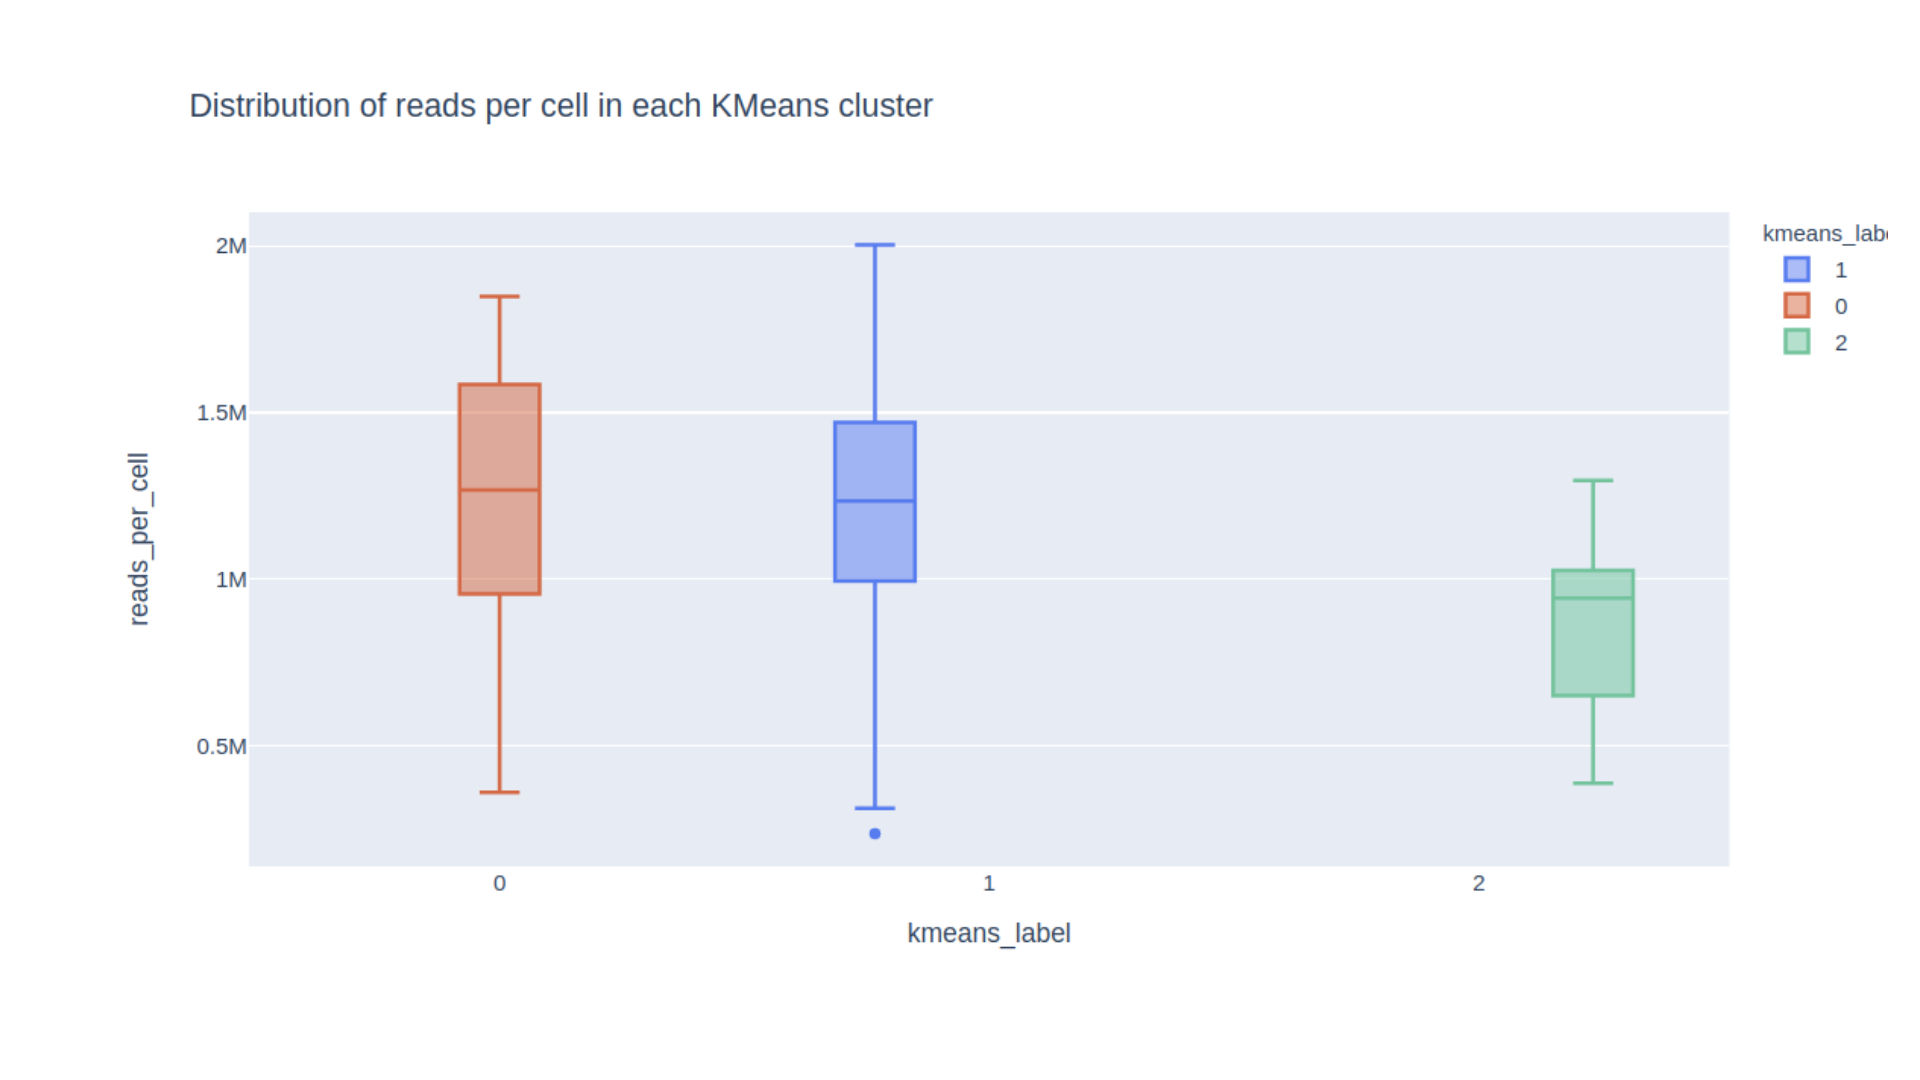
\includegraphics[keepaspectratio=true,scale=.25]{images/stp_nuclei_major_clones_read_depth_boxplots.png}
	\caption{Распределения глубины прочтений в клетках клональных линий, полученных иерархической кластеризацией мутационных профилей, предсказанных CellRanger. STP-Nuclei, scDNA-seq. 0 — тетраплоидные>> клеток опухоли, 1 — <<диплоидные>> клетки опухоли, 2 — нормальные клетки. Видно, что глубина покрытия у опухолевых клеток значимо выше, чем у нормальных, но между собой два класса опухолевых клеток почти не отличаются.}
\end{figure}

Наблюдения хорошо согласовывались с теоретической моделью XClone-V2. Запуск на данных STP-Nuclei дал следующий результат: 

\begin{figure}[H]
	\centering
	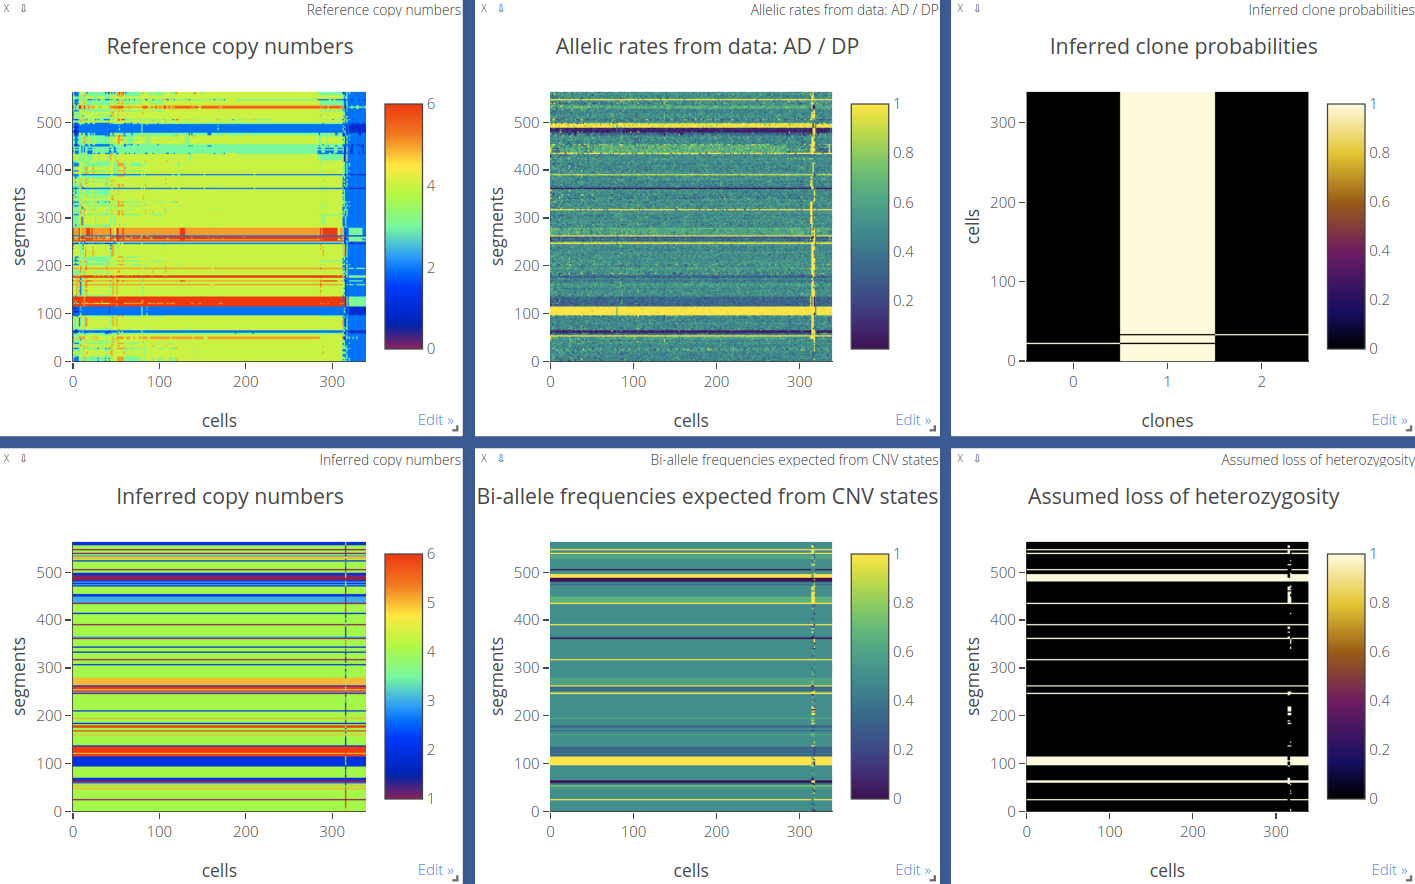
\includegraphics[keepaspectratio=true,scale=.3]{images/xclone_v2_stp_nuclei_results.png}
	\caption{Результаты запуска XClone-V2 (только опухолевые клетки). STP-Nuclei, scDNA. Верхняя строка, слева направо: число копий, предсказанное CHISEL; аллельный дисбаланс в данных; вероятности клональных линий (строки — клетки, столбцы — метки). Нижняя строка, слева направо: предсказанное число копий; предсказанный аллельный дисбаланс (определяется ASCNV); маска утраты гетерозиготности (по предсказанным ASCNV)}
\end{figure}

Как и ожидалось, алгоритм находит только одну клональную линию. Тем не менее, аллель-зависимые структурные вариации в ней метод находит правдоподобные. 

\begin{figure}[H]
	\centering
	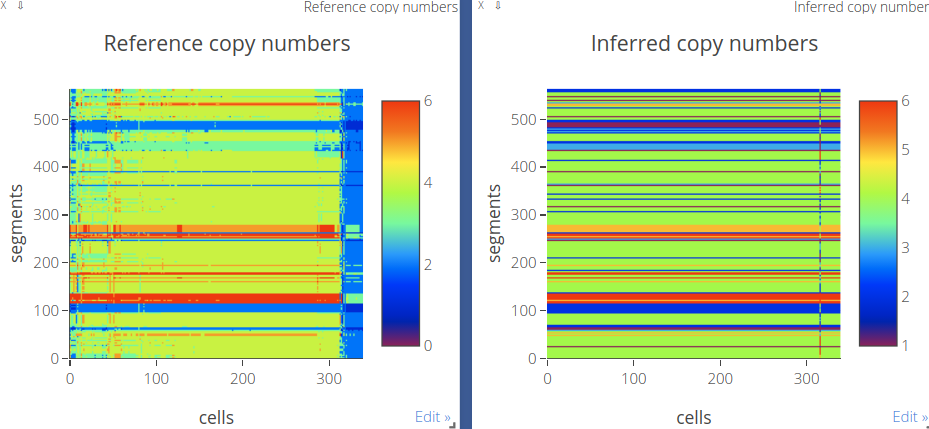
\includegraphics[keepaspectratio=true,scale=.5]{images/xclone_v2_stp_nuclei_chisel_vs_xclone.png}
	\caption{Сравнение числа копий, предсказанного CHISEL и XClone-V2. STP-Nuclei, scDNA. С точностью до WGD, структурные вариации согласуются.}
\end{figure}

Учитывая, что результаты CHISEL и CellRanger на этих данных особо не отличаются, можно заключить, что три метода дают согласованный результат. Безусловно, это не полноценное сравнение трёх методов, оно только предстоит и будет обязательно проведено, когда:
\begin{itemize}
	\item Будут исправлены известные недостатки XClone-V2;
	\item Будет найден образец с клональной структурой, достоверно известной до мелочей.
\end{itemize} 
Обзорных статей по сравнению методов детекции CNV по данным single-cell секвенирования, в целом, мало, т.к. это относительно новая и пока мало изученная задача, но перед публикацией такой анализ обязательно будет проведен.

\begin{figure}[H]
	\centering
	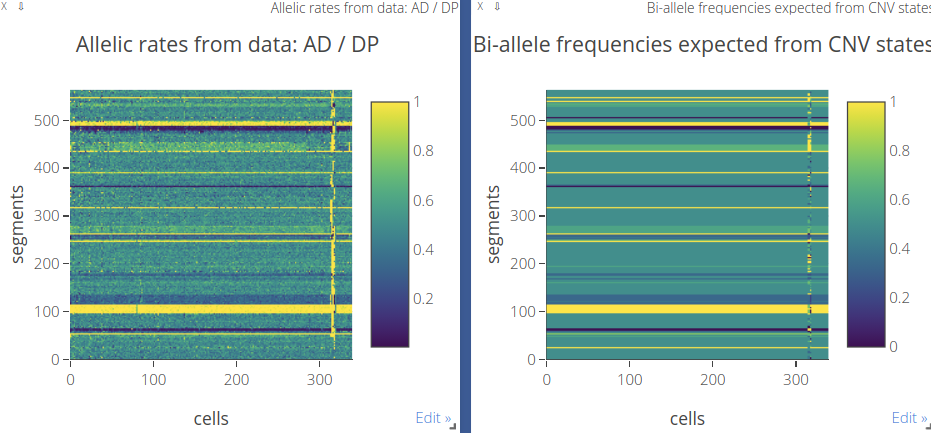
\includegraphics[keepaspectratio=true,scale=.5]{images/xclone_v2_stp_nuclei_true_vs_inferred_bafs.png}
	\caption{Сравнение числа копий, предсказанного CHISEL и XClone-V2. STP-Nuclei, scDNA. С точностью до WGD, структурные вариации согласуются.}
\end{figure}

Предсказанные ASCNV с высокой точностью воспроизводят наблюдаемую картину аллельного дисбаланса в образце. Вместе с результатами, полученными на синтетических данных, это демонстрирует, что направление исследований перспективное, а алгоритм, в целом, рабоатет. Увы, опухоль оказалась не настолько неоднородной, как авторы долгое время предполагали, но это стало понятно довольно поздно, и будет исправлено использованием других данных на следующих итерациях разработки метода.

\subsection{Реальные данные: STP, scRNA-seq}
Как уже упоминалось ранее, изначально XClone задумывался как метод совместного анализа нескольких омик. В планах было увязать друг с другом хотя бы геномные и транскриптомные данные: определять клональную структуру опухоли по scDNA-seq, а потом классифицировать по клональным линиям клетки последовательных scRNA-seq образцов и следить за эволюцией опухоли в динамике. Это позволило бы лучше понимать, как опухоль реагирует на лечение. Если бы метод работал надёжно, то он мог бы стать ценным инструментом в руках врачей-онкологов.

Но интеграция нескольких single-cell омик неспроста считается одной из 11 главных задач анализа single-cell данных \cite{ElevenGrandChallengesInSingleCellDS}. Первые результаты выглядели вдохновляюще:

\begin{figure}[H]
	\centering
	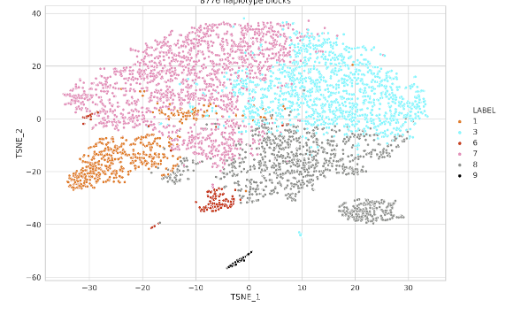
\includegraphics[keepaspectratio=true,scale=0.8]{images/xclone_v1_stp_nuclei_rna_clones_tsne.png}
	\caption{Клетки РНК-образца, STP-Nuclei. Цвет соответствует клональной линии, предсказанной XClone-V1. Большой кластер точек по центру — опухолевые клетки, кластер снизу справа — нормальные клетки, природу малых кластеров в нижней части рисунка установить не удалось.}
\end{figure}

\begin{figure}[H]
	\centering
	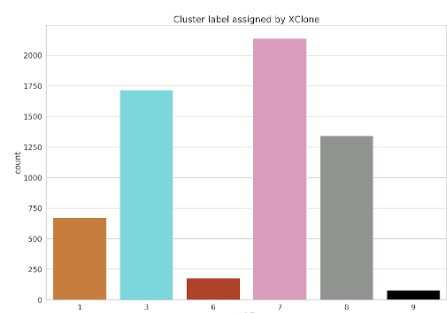
\includegraphics[keepaspectratio=true,scale=0.8]{images/xclone_v1_stp_nuclei_rna_clones_hist.png}
	\caption{Клетки РНК-образца, STP-Nuclei. Гистограммы предсказанных классов на предыдущем рисунке.}
\end{figure}

Да, часть опухолевых клеток была размечена как нормальные, но изначально это списали на то, что в данных могла быть примесь других клеточных типов, которые по профилю транскрипции находятся где-то между нормальными и опухолевыми. Тем не менее, систематический перебор random seed показал, что пропорции предсказанных классов, равно как и их количество и размеры, меняются в слишком больших пределах. Проще говоря, траскриптомных данных было слишком мало, чтобы получить достаточно хороший BAF-сигнал. 

Предпринималось много попыток сгруппировать гетерозиготные ОНП так, чтобы суммарный сигнал был достаточно сильным для уверенной классификации. Тем не менее, все они упирались в проблемы статистического фазирования гаплотипов, причём как статистического, так и основанного на длинных прочтениях, полученных по технологии Oxford Nanopore. Тем не менее, работа продолжалась. Большие надежды возлагались на разработанный метод коррекции ошибок смены цепи, который зарекомендовал себя на данных scDNA-seq образцов STP-Nuclei и STP-G\&T.

Тем не менее, scRNA-seq данные STP-Nuclei оставались слишком разреженными даже в масштабе десятков мегабаз, когда предсказание числа копий уже теряло содержательный смысл:

\begin{figure}[H]
	\centering
	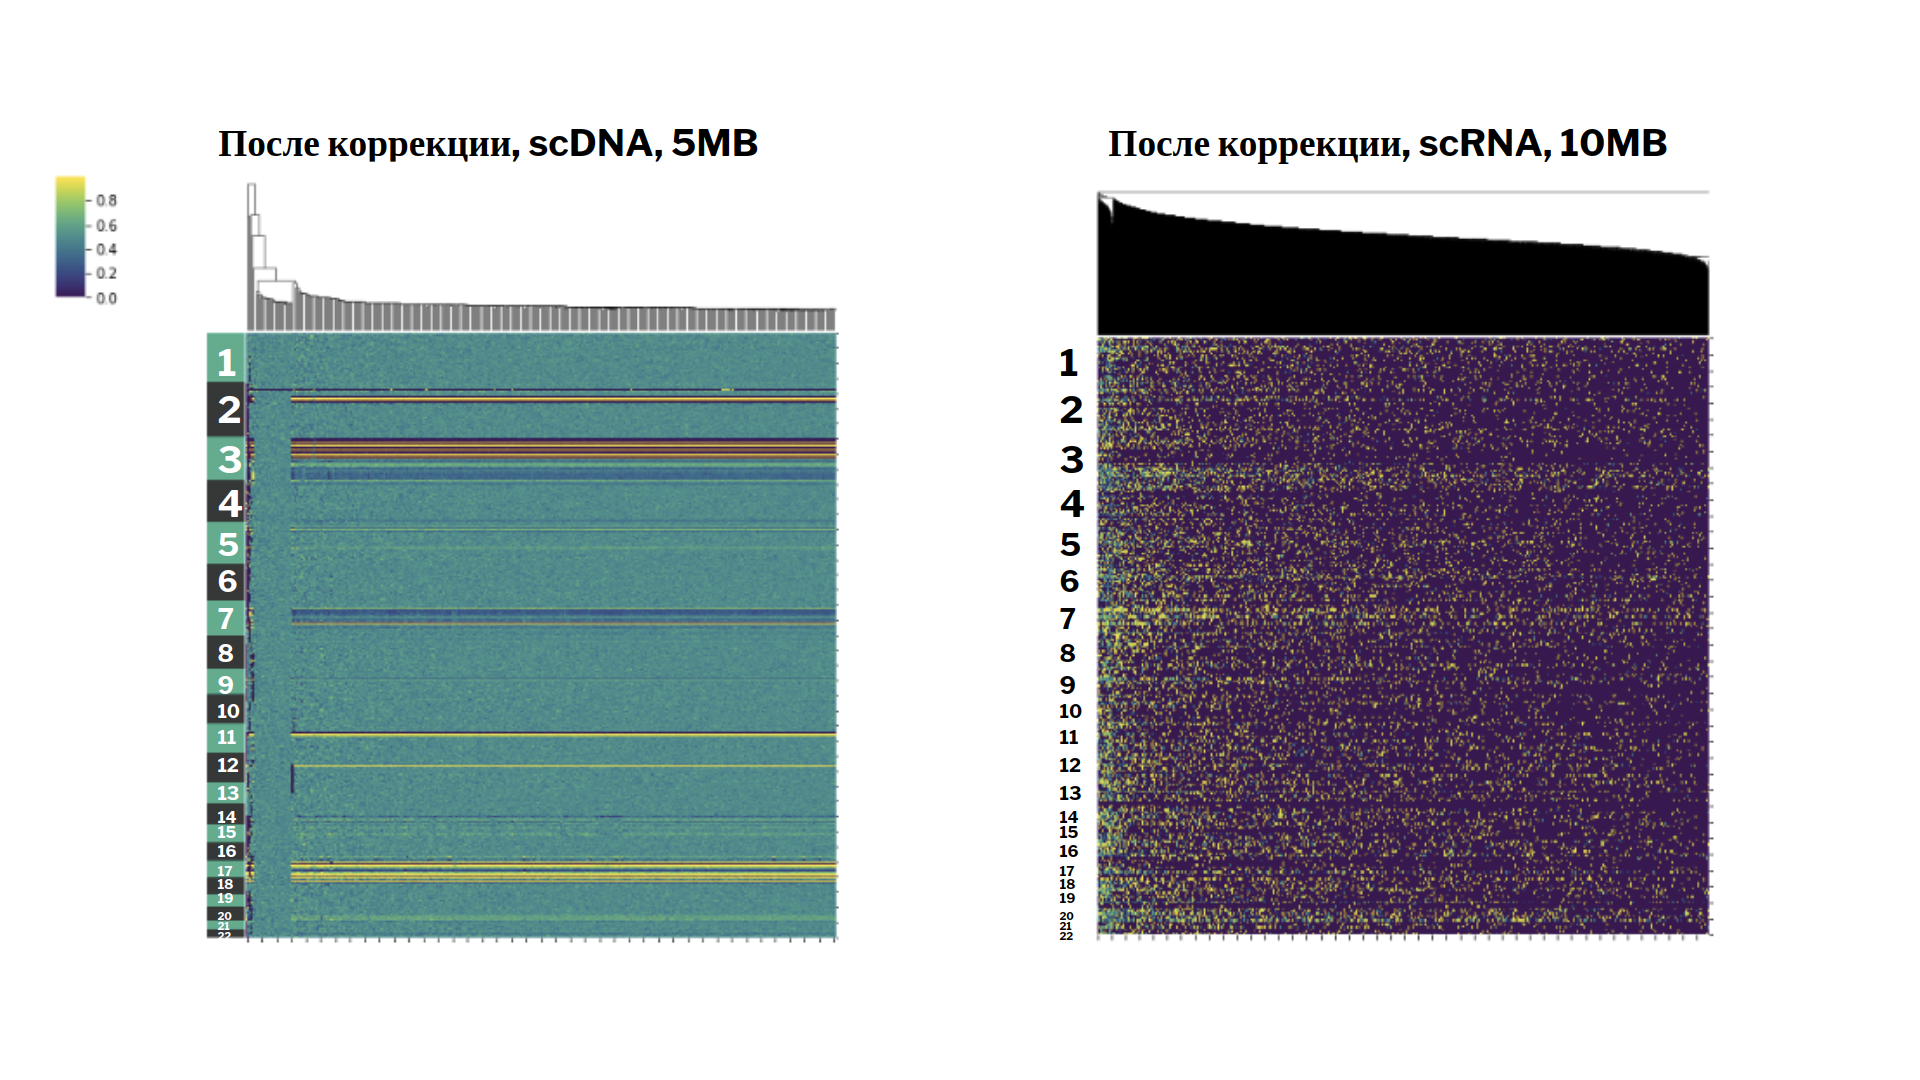
\includegraphics[keepaspectratio=true,scale=0.325]{images/bin_linkage_stp_nuclei_dna_rna.png}
	\caption{Попытка коррекция ошибок смены цепи на примере ДНК- и РНК-образцов медуллобластомы, STP-Nuclei. Здесь фиолетовый цвет означает "нет данных". Даже в масштабе 10 мегабаз структура аллельного дисбаланса в данных РНК-секвенирования практически не просматривается.}
\end{figure}

Несмотря на то, что РНК-данные из STP-G\&T гораздо менее разреженные, чем РНК-данные из STP-Nuclei, структура аллельного дисбаланса в них тоже не просматривалась:

\begin{figure}[H]
	\centering
	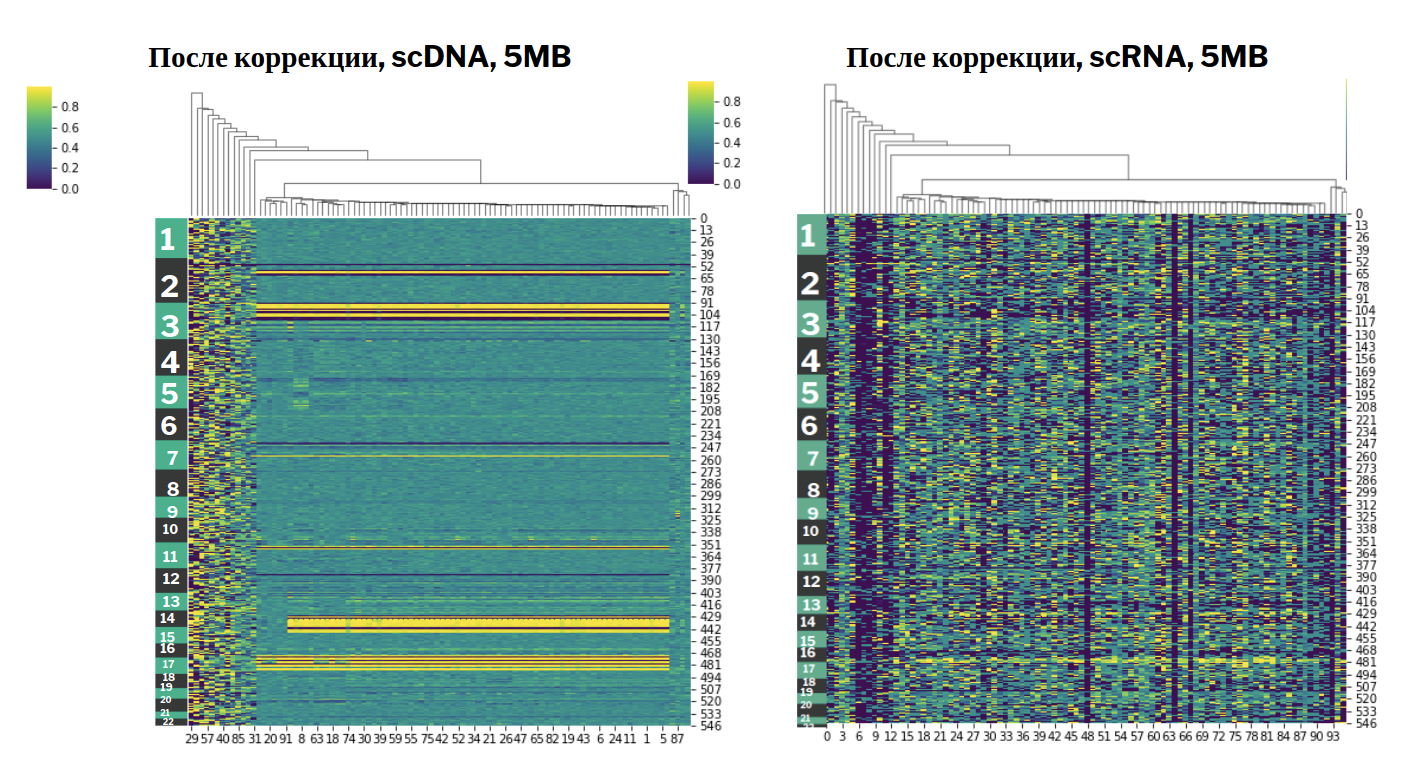
\includegraphics[keepaspectratio=true,scale=0.325]{images/bin_linkage_stp_gt_dna_rna.png}
	\caption{Попытка коррекция ошибок смены цепи на примере ДНК- и РНК-образцов медуллобластомы, STP-G\&T. Порядок клеток одинаков на обеих тепловых картах.}
\end{figure}

С похожими проблемами столкнулись и авторы алгоритма CaSpER\cite{CaSpER}. Ожидать, что много научных групп сможет позволить себе глубокое scRNA-секвенирование не приходится. Как следствие, было принято решение сосредоточиться на получении RDR-сигнала из РНК-данных. Перспективность этой гипотезы подтверждается картиной loss/gain-событий, которую предсказывает алгоритм InferCNV:

\begin{figure}[H]
	\centering
	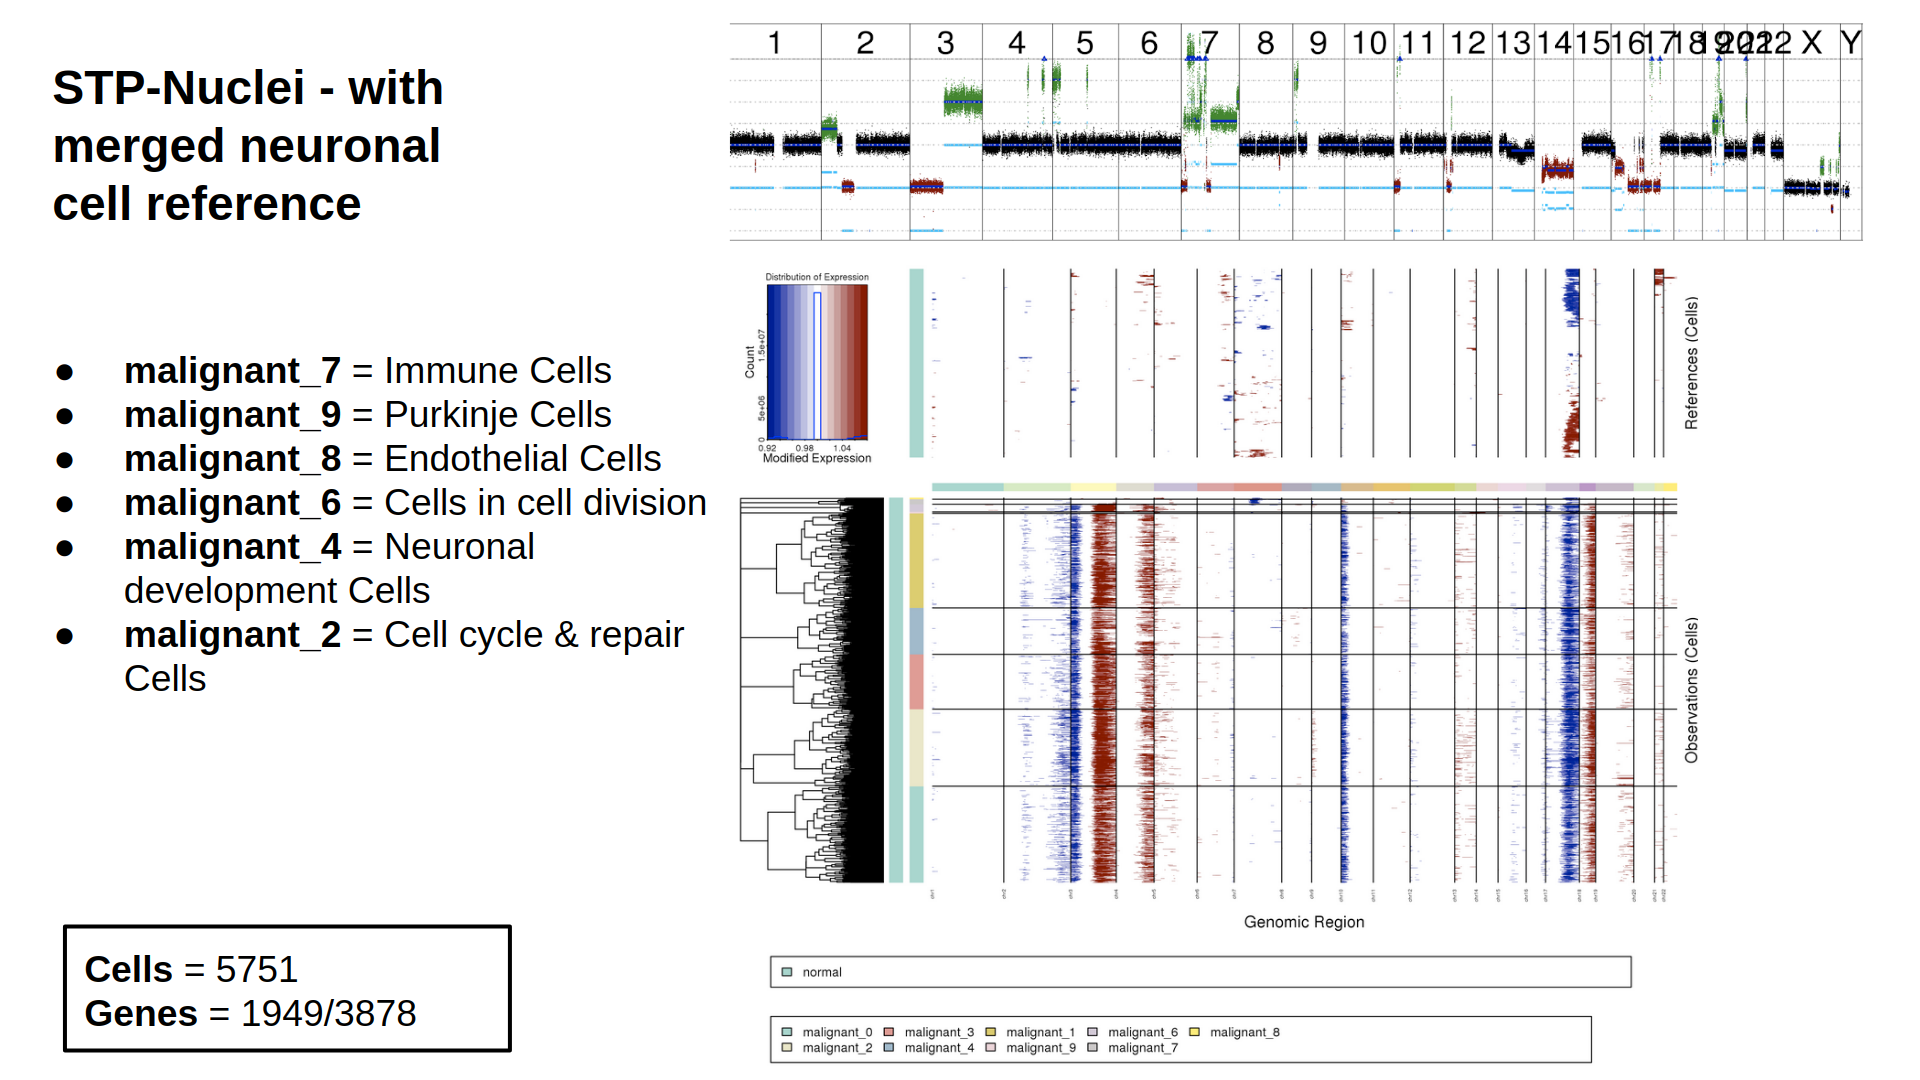
\includegraphics[keepaspectratio=true,scale=0.25]{images/infercnv_stp_nuclei.png}
	\caption{Loss-/gain- события, предсказанные алгоритмом InferCNV по scRNA-seq образцу STP-Nuclei. Видны основные клональные события: делеция p-плеча и амплификация q-плеча хромосомы 3, хромотрипсис на хромосоме 7, делеции на хромосомах 14 и 16-17. Несмотря на то, что в образце 5751 клетка, опухоль всё ещё выглядит однородной, что подтверждает наблюдения, полученные по ДНК-образцу этой же опухоли.}
\end{figure}

Да, алгоритм InferCNV не совершенен, предсказывает только loss/gain-метку, но не число копий, и сильно зависит от качестве эталонного профиля экспрессии в нормальных клетках. В онкологической практике нормальную ткань часто не секвенируют, а базы данных, к которой можно было бы обратиться, нет. Точнее, пока нет: в проекте <<Human Cell Atlas>>\cite{HumanCellAtlas} уже не первый год ведётся активная работа по сбору и систематизации данных обо всех типах клеток человека. Тем не менее, single-cell секвенирования это молодая технология, атлас не завершён даже для нормальных клеток, что уже говорить о всевозможных патологиях. Кроме того, уровни экспрессии сильно зависят от множества факторов: стадия клеточного цикла, состояние окружающей среды, возраст клетки, состояние ткани... Это т.н. batch effect, и без поправок на него невозможно сравнивать результаты, полученные по данным из разных образцов. Устранение влияния технических факторов тоже считается одной из 11 главных задач анализа sigle-cell данных\cite{ElevenGrandChallengesInSingleCellDS}.

При всём при этом метод дарит надежду, что при известной клональной структуре, предсказанной по ДНК-образцу той же опухоли, можно будет разметить и клетки РНК-образца, используя RDR-сигнал, подсчитанный при аналогичной многостадийной предобработке данных. Достаточно было бы просто выбрать ту клональную линию, RDR-профиль которой наиболее похож (в смысле максимизации правдоподобия в модели, полученной при адаптации RDR-модуля из XClone). В момент написания этого текста ведётся активная работа в данном направлении.
